\def\mytitle{MATRICES USING PYTHON}
\def\myauthor{THOUTU RAHUL RAJ}
\def\contact{rdj4648@gmail.com}
\def\mymodule{Future Wireless Communication (FWC)}
\documentclass[10pt, a4paper]{article}
\usepackage[a4paper,outer=1.5cm,inner=1.5cm,top=1.75cm,bottom=1.5cm]{geometry}
\twocolumn
\usepackage{graphicx}
\graphicspath{{./images/}}
\usepackage[colorlinks,linkcolor={black},citecolor={blue!80!black},urlcolor={blue!80!black}]{hyperref}
\usepackage[parfill]{parskip}
\usepackage{lmodern}
\usepackage{amsmath,amsfonts,amssymb,amsthm}
\usepackage{tikz}
	\usepackage{physics}
%\documentclass[tikz, border=2mm]{standalone}
\usepackage{karnaugh-map}
%\documentclass{article}
\usepackage{tabularx}
\usepackage{circuitikz}
\usetikzlibrary{calc}
\usepackage{amsmath}
\usepackage{amssymb}
\renewcommand*\familydefault{\sfdefault}
\usepackage{watermark}
\usepackage{lipsum}
\usepackage{xcolor}
\usepackage{listings}
\usepackage{float}
\usepackage{titlesec}
\providecommand{\norm}[1]{\left\lVert#1\right\rVert}
\providecommand{\sbrak}[1]{\ensuremath{{}\left[#1\right]}}
\providecommand{\lsbrak}[1]{\ensuremath{{}\left[#1\right.}}
\providecommand{\rsbrak}[1]{\ensuremath{{}\left.#1\right]}}
\providecommand{\brak}[1]{\ensuremath{\left(#1\right)}}
\providecommand{\lbrak}[1]{\ensuremath{\left(#1\right.}}
\providecommand{\rbrak}[1]{\ensuremath{\left.#1\right)}}
\providecommand{\cbrak}[1]{\ensuremath{\left\{#1\right\}}}
\providecommand{\lcbrak}[1]{\ensuremath{\left\{#1\right.}}
\providecommand{\rcbrak}[1]{\ensuremath{\left.#1\right\}}}
\newcommand{\myvec}[1]{\ensuremath{\begin{pmatrix}#1\end{pmatrix}}}
\let\vec\mathbf
\providecommand{\mtx}[1]{\mathbf{#1}}
\titlespacing{\subsection}{1pt}{\parskip}{3pt}
\titlespacing{\subsubsection}{0pt}{\parskip}{-\parskip}
\titlespacing{\paragraph}{0pt}{\parskip}{\parskip}
\newcommand{\figuremacro}[5]

\begin{document}

\title{\mytitle}
\author{\myauthor\hspace{1em}\\\contact\\FWC22008\hspace{6.5em}IITH\hspace{0.5em}\mymodule\hspace{6em}ASSIGN-4}
\date{}
	\maketitle
		
	\tableofcontents
\vspace{5mm}
   \section{Problem}
\paragraph{ If diagonals of a parallelogram are equal then show that it is a rectangle }
   \section{Solution}
   \textbf{Theory:}\\

   Given  ABCD is a parallelogram and AC = BD \\ 

\textbf{To Prove:} It is a rectangle.\\
Rectange is a parallelogram with all its interior angles as 90 degrees. As given all diagonals are equall so if we prove anyone angle in the triangle is 90 then it will automatically become rectangle.\\
\\
In $\Delta$ ABC and $\angle$ DCB   \\
AB = DC (opposite sides of parallelogram are equal) \\
\\
 BC = BC (Common)\\
   \\
   AC = DB (Given)\\
 \\ 
$\triangle ABC$ $\cong$ $\triangle DCB$ are congruent to each other by SSS congruency.  \\
 \\ 
 therefore $\angle$ ABC = $\angle$ DCB (CPCT)\\
 \\
 \\
Now,
 %\vspace{10mm}
 AB $\parallel$ BC \\
 \\
 And BC is a transversal
 Therefore $\angle$ B + $\angle$ C = 180 $\deg$(interior angles on the same side of transversal are supplementary)\\
 \\
 $\angle$B + $\angle$B = 180 $/deg$\\
 \\
  2$\angle$B = 180 $\deg$\\
 \\
 $\angle$B = 90 $\deg$\\
 AD=DC \\
 
 Therefore $\angle$ DAC= $\angle$ DCA\\
 
\vspace{1mm}
\textbf{Termux commands :}
\begin{lstlisting}
python3 matrixline.py
\end{lstlisting}


The input parameters for this construction are 
\begin{center}
\begin{tabular}{|c|c|c|}
	\hline
	\textbf{Symbol}&\textbf{Value}&\textbf{Description}\\
	\hline
	r&6&AC\\
	\hline
	k&4&AB\\ 
	\hline
	${\theta}$& arccos(k/r)&$ \angle $AC\\
	\hline
	\textbf{A}&$\
	\begin{pmatrix}
		0 \\
		0 \\
	\end{pmatrix}$%
	&Point A\\
	\hline
	
\end{tabular}
\end{center}
\vspace{.25 cm}
\textbf{To Prove:}\\ 
ABCD is a rectangle\\
\\
Given
\begin{align}
 \vec{AC} = \vec{BD} 
\end{align}
By Triangle law of vector addition
\begin{align}
\vec{AC} = \vec{AD} + \vec{DC}\\
= \vec{AD-CD} \\
 = \vec{BC} - \vec{CD}\\
\vec{BD} = \vec{BC} + \vec{CD}\\
\end{align}
\begin{align}
 \vec{a1} = \vec{C} - \vec{B}\\
 \vec{a2} = \vec{C} - \vec{D}
	\end{align}
	%a1=A-B\\
	%a2=A-D\\
	
`Angle between vectors a1,a2 is given by \\
\begin{align}
\cos \theta =\frac{\mathbf{(D-C)}^T  \mathbf{(C-B)}}{\norm{\vec{(B-C)}}\norm{\vec{(C-D)}}}
	\end{align}
\vspace{3mm}\\
\begin{align}
cos\theta = 0\\
\theta = 90\deg
\end{align}
$\therefore$ It is a rectangle\\

 \section{Construction}
 	\begin{center}
     Figure of Construction
     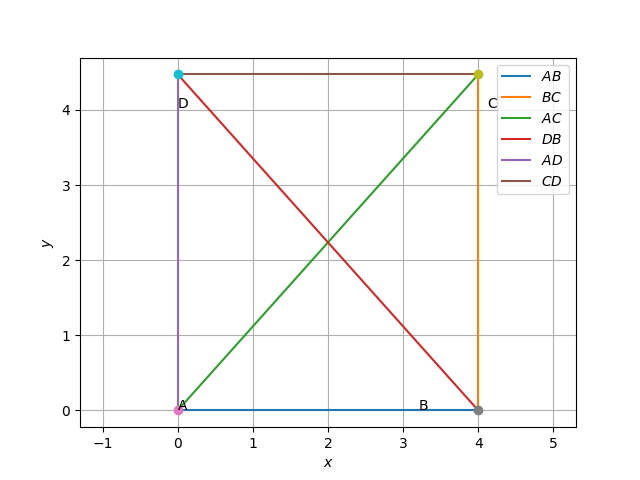
\includegraphics[scale=0.5]{fig.png}
  	\end{center}
  	\vspace{1mm}
The below python code realizes the above construction:	\\
\url{https://github.com/Rahulraj00/Assignments/tree/main/Assignments/assg_4}
\bibliographystyle{ieeetr}
\end{document}